\documentclass[noanswer,fancy,blue,11pt]{elegantbook}

\title{An Elegant \LaTeX{} Template for Books}
\subtitle{Classic Elegant\LaTeX{} Template}

\author{Ethan Deng \& Liam Huang}
\institute{Elegant\LaTeX{} Program}
\date{\today}
\version{3.07}

\equote{Victory won\rq t come to us unless we go to it. --- M. Moore}

\logo{logo.png}
\cover{cover.jpg}



\begin{document}

\maketitle
\tableofcontents
\clearpage
\thispagestyle{empty}
\mainmatter
\hypersetup{pageanchor=true}

\chapter{Elegant\LaTeX{} Templates}

On the occasion of this release, we, Elegant\LaTeX{} Program, want to reintroduce our work to you. We are committed to creating a series of beautiful, elegant, easy to use \LaTeX{} templates for users. The Elegant\LaTeX{} is currently composed of \href{https://github.com/ElegantLaTeX/ElegantNote}{ElegantNote}, \href{https://github.com/ElegantLaTeX/ElegantBook}{ElegantBook}, \href{https://github.com/ElegantLaTeX/ElegantPaper}{ElegantPaper} for typesetting notes, books, and working papers respectively. 

The latest version is available on \href{https://github.com/ElegantLaTeX/ElegantBook/releases}{Github}. This guide describes some settings of this template and how to use it. If you have any other questions, suggestions or comments, please feel free to contact us, our email is \email{elegantlatex2e@gmail.com}.


\section{ElegantBook Updates}
Over these years, we've received a lot of feedbacks from users, with major issues related to font installation, coding support, theorem class environments floats, theorem cross-page, cross-references, and etc. We really think about these problems, it wasn't elegant to let the user install the font for visual beauty since users got into a lot of trouble, which went against the concept of our template. So we've removed that from the new version, users don't have to install any fonts. Let's take a look at the ElegantBook template 3.x updates:

\begin{enumerate}
   \item Remove custom font settings;
   \item Add English and Chinese modes;
   \item \lstinline{PDFLaTeX} and \lstinline{XeLaTeX} support;
   \item Use the \lstinline{tcolorbox} package to re-written the theorem class environments;
   \item Theorem class environments name updated, and cross-references fixed;
   \item renew color themes and add gray and black theme;
   \item Color name updated, link color unified;
   \item New Elegant\LaTeX{} Logo;
   \item New cover and decorations, remove the watermark;
   \item Fix appendix;
   \item Add code highlighting;
   \item Beautify the list environments;
   \item Add simple theorem mode;
   \item Add base hide option.
\end{enumerate}


\chapter{ElegantBook Settings}


\section{Compilation Methods}
This template is based on the Standard LaTeX book class,  so the options of book class also work. The default encoding is UTF-8, and \TeX{} Live is recommended. The test environment is Win10 + \TeX{} Live 2018. 


\section{Languages}

We defined one option named \lstinline{lang}, this option has two alternative values, \lstinline{lang=en} (default) or \lstinline{lang=cn}. \lstinline{lang=cn} will make the captions of figure/table, abstract name, refname etc. Chinese. You can use this option as
\begin{lstlisting}
\documentclass[en]{elegantbook} 
\documentclass[lang=en]{elegantbook}
\end{lstlisting}

\begin{remark}
You can input Chinese Characters in either \lstinline{lang=en} or \lstinline{lang=cn}. If you are using (\lstinline{lstlisting}) environment, and it contains Chinese characters, please use \lstinline{XeLaTeX}.
\end{remark}


\section{Color Themes}
This template contains 5 color themes,they are  \textcolor{main1}{\lstinline{green}}\footnote{original default theme.}, \textcolor{main2}{\lstinline{cyan}}, \textcolor{main3}{\lstinline{blue}}(default), \textcolor{main4}{\lstinline{gray}}, \textcolor{main5}{\lstinline{black}}. You can choose \lstinline{green} with  
\begin{lstlisting}
\documentclass[green]{elegantbook} %or
\documentclass[color=green]{elegantbook}
\end{lstlisting}


\begin{table}[htbp]
\caption{ElegantBook Themes\label{tab:color thm}}
\centering
\begin{tabular}{ccccccc}
\toprule
	        & \textcolor{main1}{green} 
	        & \textcolor{main2}{cyan} 
	        & \textcolor{main3}{blue}
	        & \textcolor{main4}{gray} 
	        & \textcolor{main5}{black} 
	        & Main Environments\\
\midrule
structure & \makecell{{\color{structure1}\rule{1cm}{1cm}}}
				& \makecell{{\color{structure2}\rule{1cm}{1cm}}}
				& \makecell{{\color{structure3}\rule{1cm}{1cm}}} 
				& \makecell{{\color{structure4}\rule{1cm}{1cm}}} 
				& \makecell{{\color{structure5}\rule{1cm}{1cm}}} 
				& chapter  section  subsection \\
main      & \makecell{{\color{main1}\rule{1cm}{1cm}}}
				& \makecell{{\color{main2}\rule{1cm}{1cm}}}
				& \makecell{{\color{main3}\rule{1cm}{1cm}}}
				& \makecell{{\color{main4}\rule{1cm}{1cm}}}
				& \makecell{{\color{main5}\rule{1cm}{1cm}}}
				& definition  exercise  problem  \\
second    & \makecell{{\color{second1}\rule{1cm}{1cm}}}
				& \makecell{{\color{second2}\rule{1cm}{1cm}}}
				& \makecell{{\color{second3}\rule{1cm}{1cm}}}
				& \makecell{{\color{second4}\rule{1cm}{1cm}}}
				& \makecell{{\color{second5}\rule{1cm}{1cm}}}
				& theorem  lemma  corollary\\
third     & \makecell{{\color{third1}\rule{1cm}{1cm}}}
				& \makecell{{\color{third2}\rule{1cm}{1cm}}}
				& \makecell{{\color{third3}\rule{1cm}{1cm}}}
				& \makecell{{\color{third4}\rule{1cm}{1cm}}}
				& \makecell{{\color{third5}\rule{1cm}{1cm}}}
				& proposition\\
\bottomrule
\end{tabular}
\end{table}

If you want to customize the colors, please select \lstinline{nocolor} or use \lstinline{color=none} , then define the main, second, and third colors in the preamble section as follows:
\begin{lstlisting}[frame=single]
\definecolor{structurecolor}{RGB}{60,113,183}
\definecolor{main}{RGB}{0,166,82}%
\definecolor{second}{RGB}{255,134,24}%
\definecolor{third}{RGB}{0,174,247}% 
\end{lstlisting}


\section{Chapter Title Display Styles}

This template contains 2 sets of \textit{title display styles},which including \lstinline{hang}(default) and \lstinline{display} style, 

The difference is that the chapter heading is displayed on a single line (\lstinline{hang}) and on a double line (\lstinline{display}) , and this guide uses \lstinline{hang} . To change display style
\begin{lstlisting}
\documentclass[hang]{elegantbook} %or
\documentclass[titlestyle=hang]{elegantbook}
\end{lstlisting}

\section{Theorem Class Environments}
We defined two sets of theorem modes, \lstinline{simple} style and \lstinline{fancy} style (default), you can change to \lstinline{simple} mode by 
\begin{lstlisting}
\documentclass[simple]{elegantbook} %or
\documentclass[mode=simple]{elegantbook}
\end{lstlisting}

In this template, we defined four categories of theorem class environments

\begin{itemize}
\item \textit{Theorem Environment}, including title and contents, numbering within chapter. There are three types depending on the format
   \begin{itemize}
      \item \textcolor{main}{\textbf{definition}} environment, the color is  \textcolor{main}{main};
      \item \textcolor{second}{\textbf{theorem, lemma, corollary}} environment, the color is \textcolor{second} {second};
      \item \textcolor{third}{\textbf{proposition}} environment, the color is \textcolor{third}{third}.
   \end{itemize}
\item \textit{Example Environments}, including \textbf{example, exercise, problem} environment, auto numering within chapter.
\item \textit{Proof Environment}, including \textbf{proof, note} environment, they contain introductory symbol (\textbf{note} environment) or ending symbol (\textbf{proof} environment).
\item \textit{Conclusion Environments}, including \textbf{conclusion, assumption, property, remark, solution}\footnote{We also define and key \lstinline{result}, which can hide the \lstinline{solution} and \lstinline{proof} environments. You can switch by \lstinline{result=answer} or \lstinline{result=noanswer}} environment, all of these begin with boldfaced words, and the contents are the same as a normal paragraph.
\end{itemize}

\subsection{Theorem Class Environments}
The template uses the \lstinline{tcolorbox} package to customize the theorem class environments, it is slightly different from the normal theorem environments. The usage is as follows:
\begin{lstlisting}
\begin{theorem}{<theorem name>}{<label>}
The content of theorem.
\end{theorem}
\end{lstlisting}

The first parameter \lstinline{<theorem name>} is the name of the theorem, and the second parameter \lstinline{label} is the label used in cross-reference with \verb|ref{thm:label}|. Note that cross-references must be prefixed with \lstinline{thm:}. 

Other theorem class environments with the same usage are:

\begin{table}[htbp]
   \centering
   \caption{Theorem Class Environments}
     \begin{tabular}{llll}
     \toprule
     Environment & Label text & Prefix & Cross-reference \\
     \midrule
     definition & label & def   & \lstinline|\ref{def:label}| \\
     theorem & label & thm   & \lstinline|\ref{thm:label}| \\
     lemma & label & lem   & \lstinline|\ref{lem:label}| \\
     corrlary & label & cor   & \lstinline|\ref{cor:label}| \\
     proposition & label & pro   & \lstinline|\ref{pro:label}| \\
     \bottomrule
     \end{tabular}%
   \label{tab:theorem-class}%
 \end{table}%
 

\subsection{Other Customized Environments}
The other three math environments can be used directly since there are no options for them, the \lstinline{example} environment usage:
\begin{lstlisting}
\begin{example}
This is the content of example environment.
\end{example}
\end{lstlisting}

The effect is as follows:

\begin{example}
This is the content of example environment.
\end{example}

These are all the same environments, except that

\begin{itemize}
   \item example, exercise, problem environments numbering within chapter;
   \item note with introductory symbol, proof with ending symbol;
   \item conclusion environment with boldfaced keywords and normal paragraph content.
\end{itemize}

\section{Base Hide Option}
We defined an option to hide the base below the chapter, you can use it by
\begin{lstlisting}
\documentclass[hide]{elegantbook} %or
\documentclass[base=hide]{elegantbook}
\end{lstlisting}


\section{Cover and Logo}

The cover image used in this template is from \href{https://pixabay.com/en/tea-time-poetry-coffee-reading-3240766/}{pixabay.com}\footnote{Thank China\TeX{} for providing free image source site, and \href{https://www.pexels.com/}{pexels.com} is also recommended.}. The image is completely free and can be used in any circumstance. The cover image size is $1280 \times 1024$, when changing the cover, please crop it according to the size of the cover picture strictly. Here is a free online image clipping site: \href{https://www.befunky.com/create/crop-photo/}{befunky.com}.

This Logo ratio is 1:1, that is square picture. In the replacement of the picture, please choose the appropriate picture to replace.

\section{List Environments}
This template uses \lstinline{tikz} to customize \lstinline{itemize} and \lstinline{enumerate} environments, the \lstinline{itemize} environment customized to the third depth, and \lstinline{enumerate} environment customized to fourth depth. The effect is as follows\\[2ex]
\begin{minipage}[b]{0.49\textwidth}
\begin{itemize}
   \item first item of nesti;
   \item second item of nesti;
   \begin{itemize}
      \item first item of nestii;
      \item second item of nestii;
      \begin{itemize}
         \item first item of nestiii;
         \item second item of nestiii.
      \end{itemize}   
   \end{itemize}
\end{itemize}
\end{minipage}
\begin{minipage}[b]{0.49\textwidth}
\begin{enumerate}
   \item first item of nesti;
   \item second item of nesti;
   \begin{enumerate}
      \item first item of nestii;
      \item second item of nestii;
      \begin{enumerate}
         \item first item of nestiii;
         \item second item of nestiii.
      \end{enumerate}   
   \end{enumerate}
\end{enumerate}
\end{minipage}

\section{Bibliography}

This template uses \hologo{BibTeX} to generate the bibliography, the default bibliography style is \lstinline{aer}. Let's take a glance at the citation effect, ~\cite{en1} use data from a major peer-to-peer lending marketplace in China to study whether female and male investors evaluate loan performance differently. 

If you want to use \hologo{BibTeX}, you must create a file named \lstinline{reference.bib}, and add bib items (from Google Scholar, Mendeley, EndNote, and etc.) to \lstinline{reference.bib} file, and cite the bibkey in the \lstinline{tex} file. The Bib\TeX{} will automatically generate the bibliography for you for the reference you cited. If you want to add some noncited reference to the bibliography, you can use 
\begin{lstlisting}
\nocite{EINAV2010, Havrylchyk2018} 
\end{lstlisting}

\section{Preface}

If you want to add a preface before the first chapter without changing the number of chapter, you can use it before the first chapter 
\begin{lstlisting}
\chapter*{Preface}
\addcontentsline{toc}{chapter}{Preface} 
\markboth{Preface}{} 
The content of Preface.
\end{lstlisting}

\chapter{ElegantBook Writing Sample}

\begin{introduction}
\item Theorem Class Envrionments
\item Cross Reference
\item Math Environments
\item List Environments
\item Logo and Base 
\item $a^2+b^2=c^2$
\end{introduction}


\lipsum[1]
% source: https://www.maths.tcd.ie/~dwilkins/LaTeXPrimer/Theorems.html

\section{Writing Sample}

We will define the integral of a measurable function in three steps. First, we define the integral of a nonnegative simple function. Let $E$ be the measurable set in $\mathcal{R}^N$.

\begin{definition}{Left Coset}{}
Let $H$ be a subgroup of a group~$G$.  A \emph{left coset} of $H$ in $G$ is a subset of $G$ that is of the form $xH$, where $x \in G$ and $xH = \{ xh : h \in H \}$. Similarly a \emph{right coset} of $H$ in $G$ is a subset of $G$ that is of the form $Hx$, where $Hx = \{ hx : h \in H \}$
\end{definition}

\begin{note}
Note that a subgroup~$H$ of a group $G$ is itself a left coset of $H$ in $G$.
\end{note}

\lipsum[2]

\begin{theorem}{Lagrange's Theorem}{}
Let $G$ be a finite group, and let $H$ be a subgroup of $G$.  Then the order of $H$ divides the order of $G$.
\end{theorem}

\lipsum[3]

   
\begin{proposition}{Size of Left Coset}{}
Let $H$ be a finite subgroup of a group $G$.  Then each left coset of $H$ in $G$ has the same number of elements as $H$.
\end{proposition}

\begin{proof}
Let $z$ be some element of $xH \cap yH$.  Then $z = xa$ for some $a \in H$, and $z = yb$ for some $b \in H$. If $h$ is any element of $H$ then $ah \in H$ and $a^{-1}h \in H$, since $H$ is a subgroup of $G$. But $zh = x(ah)$ and $xh = z(a^{-1}h)$ for all $h \in H$. Therefore $zH \subset xH$ and $xH \subset zH$, and thus $xH = zH$.  Similarly $yH = zH$, and thus $xH = yH$, as required.
\end{proof}

\begin{figure}[htbp]
	\centering
	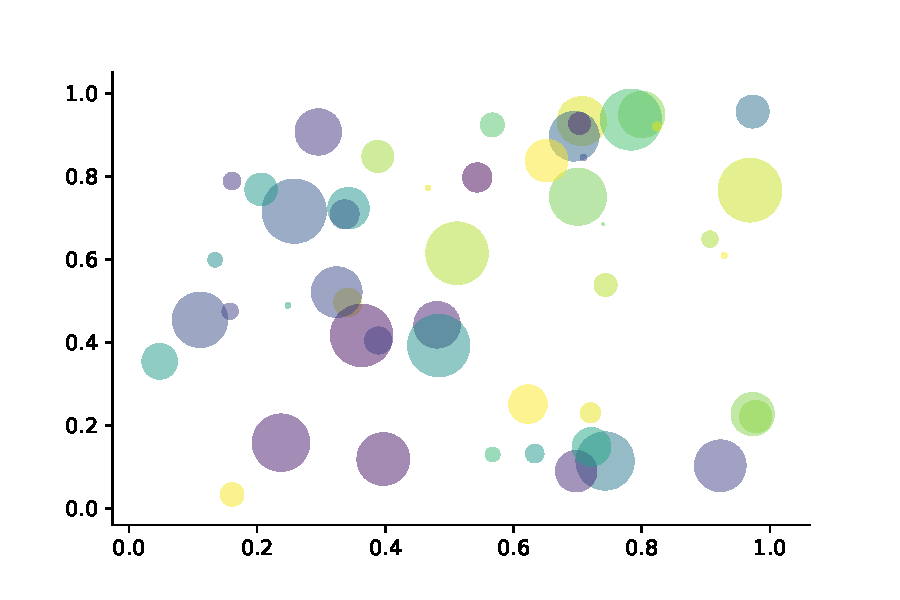
\includegraphics[width=0.6\textwidth]{scatter.pdf}
	\caption{Matplotlib: Scatter Plot Example\label{fig:scatter}}
\end{figure}

Regression analysis is a powerful statistical method that allows you to examine the relationship between two or more variables of interest. While there are many types of regression analysis, at their core they all examine the influence of one or more independent variables on a dependent variable. The process of performing a regression allows you to confidently determine which factors matter most, which factors can be ignored, and how these factors influence each other.

Let's continue using our application training example. In this case, we'd want to measure the historical levels of satisfaction with the events from the past three years or so, as well as any information possible in regards to the independent variables. 


\begin{table}[htbp]
  \small
  \centering
  \caption{Auto MPG and Price \label{tab:reg}}
    \begin{tabular}{lcc}
    \toprule
                    &       (1)         &        (2)      \\
    \midrule
    mpg             &    -238.90***     &      -49.51     \\
                    &     (53.08)       &      (86.16)    \\
    weight          &                   &      1.75***    \\
                    &                   &      (0.641)    \\
    constant        &     11,253***     &       1,946     \\
                    &     (1,171)       &      (3,597)   \\
    obs             &        74         &         74     \\
    $R^2$           &      0.220        &       0.293    \\
    \bottomrule
    \multicolumn{3}{l}{\scriptsize Standard errors in parentheses} \\
    \multicolumn{3}{l}{\scriptsize *** p<0.01, ** p<0.05, * p<0.1} \\
    \end{tabular}%
\end{table}%

\lipsum[1-2]

\begin{itemize}
	\item Routing and resource discovery;
	     \begin{itemize} 
      	   	\item Language Models
       	 	\item Vector Space Models
    		 \end{itemize}
	\item Resilient and scalable computer networks;
	\item Distributed storage and search.
\end{itemize}


\nocite{en1,en2,en3} 
\bibliography{reference}

\appendix
\chapter{Mathematical Tools}

This appendix covers some of the basic mathematics used in econometrics. We briefly discuss the properties of summation operators, study the properties of linear and some nonlinear equations, and review the ratios and percentages. We also introduce some special functions that are common in econometrics applications, including quadratic functions and natural logarithms. The first four sections require only basic algebraic techniques. The fifth section briefly reviews differential Calculus Although Calculus is not necessary to understand much of this book, it is used in some of the end-of-chapter appendices and in some of the more advanced topics in part 3.

\section{Summation Operator and Description Statistics}

\textbf{Summation Operator} is an abbreviation used to express the summation of numbers, it plays an important role in statistics and econometrics analysis. If $\{x_i: i=1, 2, \ldots, n\}$ is a sequence of $n$ numbers, the summation of the $n$ numbers is:

\begin{equation}
\sum_{i=1}^n x_i \equiv x_1 + x_2 +\cdots + x_n
\end{equation}

\chapter{A Minimal Example}

\begin{lstlisting}[frame=single]
\documentclass{elegantbook}
% title info
\title{Title}
\subtitle{Subtitle is here}
% bio info
\author{Your Name}
\institute{XXX University}
\date{\today}
% extra info
\version{1.00}
\equote{Victory won\rq t come to us unless we go to it. --- M. Moore}
\logo{logo.png}
\cover{cover.jpg}

\begin{document}

\maketitle
\tableofcontents
\mainmatter
\hypersetup{pageanchor=true}
% add preface chapter here if needed
\chapter{Example Chapter Title}
The content of chapter one.

\bibliography{reference}
\end{document}
\end{lstlisting}


\end{document}
